% -*- latex -*-
%%%%%%%%%%%%%%%%%%%%%%%%%%%%%%%%%%%%%%%%%%%%%%%%%%%%%%%%%%%%%%%%
%%%%%%%%%%%%%%%%%%%%%%%%%%%%%%%%%%%%%%%%%%%%%%%%%%%%%%%%%%%%%%%%
%%%%
%%%% This text file is part of the source of 
%%%% `Introduction to High-Performance Scientific Computing'
%%%% by Victor Eijkhout, copyright 2012/3/4/5/
%%%%
%%%% This book is distributed under a Creative Commons Attribution 3.0
%%%% Unported (CC BY 3.0) license and made possible by funding from
%%%% The Saylor Foundation \url{http://www.saylor.org}.
%%%%
%%%%
%%%%%%%%%%%%%%%%%%%%%%%%%%%%%%%%%%%%%%%%%%%%%%%%%%%%%%%%%%%%%%%%
%%%%%%%%%%%%%%%%%%%%%%%%%%%%%%%%%%%%%%%%%%%%%%%%%%%%%%%%%%%%%%%%

In this course it is assumed that you know what a matrix and a vector
are, simple algorithms such as how to multiply them, and some
properties such as invertibility of a matrix. This appendix introduces
some concepts and theorems that are not typically part of a first
course in linear algebra.

\Level 0 {Norms}

A \indexterm{norm} is a way to generalize the concept of absolute
value to multi-dimensional objects such as vectors and matrices. There
are many ways of defining a norm, and there is theory of how different
norms relate. Here we only give the basic definitions; for more detail
see any linear algebra textbook, for instance~\cite{golo83}.

\Level 1 {Vector norms}
\index{vector!norms|(}

A norm is any function $n(\cdot)$ on a vector space $V$ with the
following properties:
\begin{itemize}
\item $n(x)\geq0$ for all $x\in V$ and $n(x)=0$ only for $x=0$,
\item $n(\lambda x)=|\lambda|n(x)$ for all $x\in V$ and
  $\lambda\in\bbR$.
\item $n(x+y)\leq n(x)+n(y)$
\end{itemize}
For any $p\geq1$, the following defines a vector norm:
\[ |x|_p = \sqrt[p]{\sum_i|x_i|^p}. \]
Common norms are $\|\cdot\|_1$ (`sum of absolute values') and
$\|\cdot\|_2$ (`square root of sum of squares'); the
$\|\cdot\|_\infty$ norm is defined as
$\lim_{p\rightarrow\infty}\|\cdot\|_p$, and it is not hard to see that
this equals
\[ \|x\|_\infty=\max_i |x_i|. \]

\index{vector!norms|)}

\Level 1 {Matrix norms}
\index{matrix!norms|(}

By considering a matrix of size~$n$ as a vector of length $n^2$, we
can define the Frobenius matrix norm:
\[ \|A\|_F=\sqrt{\sum_{i,j}|a_{ij}|^2}. \]
However, we will mostly look at \emph{associated matrix
  norms}\index{matrix!norms!associated}:
\[ \|A\|_p=\sup_{\|x\|_p=1}\|Ax\|_p=
   \sup_x\frac{\|Ax\|_p}{\|x\|_p}.
\]
From their definition, it easily follows that 
\[ \|Ax\|\leq\|A\|\|x\| \]
for associated norms.

The following are easy to derive:
\begin{itemize}
\item $\|A\|_1=\max_j\sum_i|a_{ij}|$,
\item $\|A\|_\infty=\max_i\sum_j|a_{ij}|$.
\end{itemize}
By observing that $\|A\|_2=\sup_{\|x\|_2=1} x^tA^tAx$, it is not hard
to derive that $\|A\|_2$ is the maximal singular value of~$A$, which
is the root of the maximal eigenvalue of~$A^tA$.

The matrix \indexterm{condition number} is defined as
\[ \kappa(A)=\|A\|\,\|A\inv\|. \]
In the symmetric case, and using the 2-norm, this is the ratio between the largest and
smallest eigenvalue.

\index{matrix!norms|)}

\Level 0 {Gram-Schmidt orthogonalization}
\label{app:gram-schmidt}
\index{Gram-Schmidt|(}

The \acf{GS} algorithm takes a series of vectors and inductively
orthogonalizes them. This can be used to turn an arbitrary basis of a
vector space into an orthogonal basis; it can also be viewed as
transforming a matrix $A$ into one with orthogonal columns. If $Q$ has
orthogonal columns, $Q^tQ$ is diagonal, which is often a convenient
property to have.

The basic principle of the \ac{GS} algorithm
can be demonstrated with two
vectors~$u,v$. Suppose we want a vector $v'$ so that $u,v$ and $u,v'$
span the same space, but $v'\perp u$. For this we let
\[ v'\leftarrow v-\frac{u^tv}{u^tu}u. \]
It is easy to see that this satisfies the requirements.

Suppose we have an set of vectors
$u_1,\ldots,u_n$ that we want to orthogonalize. We do this by
successive applications of the above transformation:

\begin{quote}
  \begin{tabbing}
    For \=$i=1,\ldots,n$:\\
    \> For \=$j=1,\ldots i-1$:\\
    \>\>let $c_{ji}=u_j^tu_i/u_j^tu_j$\\
    \> For \=$i=1,\ldots,n$:\\
    \>\> update $u_i\leftarrow u_i-u_jc_{ji}$
  \end{tabbing}
\end{quote}

Often the vector $v$ in the algorithm above is normalized; this adds a line
\begin{quote}
  \begin{tabbing}
    $u_i\leftarrow u_i/\|u_i\|$
  \end{tabbing}
\end{quote}
to the algorithm.
\ac{GS} orthogonalization with this normalization, applied to a
matrix, is also known as the \indexterm{QR factorization}.

\begin{exercise}
  Suppose that we apply the \ac{GS} algorithm to the columns of a
  rectangular matrix~$A$, giving a matrix~$Q$. Prove that there is an
  upper triangular matrix~$R$ such that $A=QR$. (Hint: look at the
  $c_{ji}$ coefficients above.) If we normalize the
  orthogonal vector in the algorithm above, $Q$~has the additional property
  that $Q^tQ=I$. Prove this too.
\end{exercise}

The \ac{GS} algorithm as given above computes the desired result,
but only in exact arithmetic. A~computer implementation can be quite
inaccurate if the angle between $v$ and one of the $u_i$ is small. In
that case, the \acf{MGS}\index{Gram-Schmidt!modified} algorithm will
perform better:

\begin{quote}
  \begin{tabbing}
    For \=$i=1,\ldots,n$:\\
    \> For \=$j=1,\ldots i-1$:\\
    \>\>let $c_{ji}=u_j^tu_i/u_j^tu_j$\\
    \>\> update $u_i\leftarrow u_i-u_jc_{ji}$
  \end{tabbing}
\end{quote}

To contrast it with \ac{MGS}, the original \ac{GS} algorithm is also
known as \acf{CGS}.

As an illustration of the difference between the two methods, consider
the matrix
\[ A=
\begin{pmatrix}
  1&1&1\\ \epsilon&0&0\\ 0&\epsilon&0\\ 0&0&\epsilon
\end{pmatrix}
\]
where $\epsilon$ is of the order of the machine precision, so that
$1+\epsilon^2=\nobreak1$ in machine arithmetic.
%
The \ac{CGS} method proceeds as follows:
\begin{itemize}
\item The first column is of length~1 in machine arithmetic, so
  \[ q_1 = a_1 = 
  \begin{pmatrix}
    1\\ \epsilon\\ 0\\ 0
  \end{pmatrix}
  . \]
\item The second column gets orthogonalized as $v\leftarrow a_2-1\cdot
  q_1$, giving
  \[ v=
  \begin{pmatrix}
    0\\ -\epsilon\\ \epsilon\\ 0
  \end{pmatrix},
  \quad\hbox{normalized:}\quad
  q_2 = 
  \begin{pmatrix}
    0\\ -\frac{\sqrt 2}2\\ \frac{\sqrt2}2\\ 0
  \end{pmatrix}
  \]
\item The third column gets orthogonalized as $v\leftarrow
  a_3-c_1q_1-c_2q_2$, where 
  \[ 
  \begin{cases}
    c_1 = q_1^ta_3 = 1\\ c_2 = q_2^ta_3=0
  \end{cases}
  \Rightarrow v=
  \begin{pmatrix}
    0\\ -\epsilon\\ 0\\ \epsilon
  \end{pmatrix};\quad \hbox{normalized:}\quad q_3=
  \begin{pmatrix}
    0\\ \frac{\sqrt2}2\\ 0\\ \frac{\sqrt2}2
  \end{pmatrix}
  \]
\end{itemize}
It is easy to see that $q_2$ and $q_3$ are not orthogonal at all.
By contrast, the \ac{MGS} method differs in the last step:
\begin{itemize}
\item As before, $q_1^ta_3=1$, so
  \[ v\leftarrow a_3-q_1 = 
  \begin{pmatrix}
    0\\ -\epsilon\\ \epsilon\\ 0
  \end{pmatrix}.
  \]
  Then, $q_2^tv=\frac{\sqrt2}2\epsilon$ (note that $q_2^ta_3=0$
  before), so the second update gives
  \[ v\leftarrow v- \frac{\sqrt2}2\epsilon q_2=
  \begin{pmatrix}
    0\\ \frac\epsilon2\\ -\frac\epsilon2\\ \epsilon
  \end{pmatrix}
  ,\quad\hbox{normalized:}\quad
  \begin{pmatrix}
    0\\ \frac{\sqrt6}6\\ -\frac{\sqrt6}6\\ 2\frac{\sqrt6}6
  \end{pmatrix}
  \]
  Now all $q_i^tq_j$ are on the order of $\epsilon$
  for~$i\not=\nobreak j$.
\end{itemize}

\index{Gram-Schmidt|)}

\Level 0 {The power method}
\label{app:power-method}

The vector sequence 
\[ x_i = Ax_{i-1}, \]
where $x_0$ is some starting vector, is called the \indexterm{power
  method} since it computes the product of subsequent matrix powers
times a vector:
\[ x_i = A^ix_0. \]
There are cases where the relation between the $x_i$ vectors is
simple. For instance, if $x_0$ is an eigenvector of~$A$, we have for
some scalar~$\lambda$
\[ Ax_0=\lambda x_0 \qquad\hbox{and}\qquad x_i=\lambda^i x_0. \]
However, for an arbitrary vector $x_0$, the sequence $\{x_i\}_i$ is
likely to consist of independent vectors. Up to a point.

\begin{exercise}
  Let $A$ and $x$ be the $n\times n$ matrix and dimension~$n$ vector
  \[ 
  A = \begin{pmatrix}
    1&1\\ &1&1\\ &&\ddots&\ddots\\ &&&1&1\\&&&&1
  \end{pmatrix},\qquad
  x =  (0,\ldots,0,1)^t.
  \]
  Show that the sequence $[x,Ax,\ldots,A^ix]$ is an independent set
  for $i<n$. Why is this no longer true for~$i\geq n$?

  Now consider the matrix $B$:
  \[ B=\left(
  \begin{array}{cccc|cccc}
    1&1&&\\ &\ddots&\ddots&\\ &&1&1\\ &&&1\\ \hline
    &&&&1&1\\ &&&&&\ddots&\ddots\\ &&&&&&1&1\\ &&&&&&&1
  \end{array}\right),\qquad
  y = (0,\ldots,0,1)^t
  \]
  Show that the set $[y,By,\ldots,B^iy]$ is an independent set for
  $i<n/2$, but not for any larger values of~$i$.
\end{exercise}

While in general the vectors $x,Ax,A^2x,\ldots$ can be expected to be
independent, in computer arithmetic this story is no longer so clear.

Suppose the matrix has eigenvalues $\lambda_0>\lambda_1\geq\cdots
\lambda_{n-1}$ and corresponding eigenvectors~$u_i$ so that
\[ Au_i=\lambda_i u_i. \]
Let the vector~$x$ be written as
\[ x=c_0u_0+\cdots +c_{n-1}u_{n-1}, \]
then 
\[ A^ix = c_0\lambda_0^iu_i+\cdots +c_{n-1}\lambda_{n-1}^iu_{n-1}. \]
If we write this as 
\[ A^ix = \lambda_0^i\left[
    c_0u_i+c_1\left(\frac{\lambda_1}{\lambda_0}\right)^i+
    \cdots +c_{n-1}\left(\frac{\lambda_{n-1}}{\lambda_0}\right)^i
    \right],
\]
we see that, numerically, $A^ix$ will get progressively closer
to a multiple of~$u_0$, the \indextermsub{dominant}{eigenvector}. Hence,
any calculation that uses independence of the $A^ix$ vectors is likely
to be inaccurate.

\Level 0 {Nonnegative matrices; Perron vectors}
\label{app:perron}

If $A$ is a nonnegative matrix, the maximal eigenvalue has the
property that its eigenvector is nonnegative: this is the the
\indexterm{Perron-Frobenius theorem}.

\begin{theorem}
  If a nonnegative matrix $A$ is irreducible, its eigenvalues
  satisfy
  \begin{itemize}
  \item The eigenvalue $\alpha_1$ that is largest in magnitude is real
    and simple:
    \[ \alpha_1> |\alpha_2|\geq\cdots. \]
  \item The corresponding eigenvector is positive.
  \end{itemize}
\end{theorem}


\Level 0 {The Gershgorin theorem}
\label{app:gershgorin}

Finding the eigenvalues of a matrix is usually complicated. However,
there are some tools to estimate eigenvalues. In this section you will
see a theorem that, in some circumstances, can give useful information
on eigenvalues.

Let $A$ be a square matrix, and $x,\lambda$ an eigenpair: $Ax=\lambda
x$. Looking at one component, we have
\[ a_{ii}x_i+\sum_{j\not=i} a_{ij}x_j=\lambda x_i. \]
Taking norms:
\[ (a_{ii}-\lambda) \leq \sum_{j\not=i} |a_{ij}|
   \left|\frac{x_j}{x_i}\right|
\]
Taking the value of~$i$ for which $|x_i|$ is maximal, we find
\[ (a_{ii}-\lambda) \leq \sum_{j\not=i} |a_{ij}|.
\]
This statement can be interpreted as follows: 
\begin{quotation}
  The eigenvalue $\lambda$ is located in the circle around~$a_{ii}$
  with radius $\sum_{j\not=i}|a_{ij}|$.
\end{quotation}
Since we do not know for which value of~$i$ $|x_i|$ is maximal, we can
only say that there is \emph{some} value of~$i$ such that $\lambda$
lies in such a circle. This is the Gershgorin theorem.

\begin{theorem}
  Let $A$ be a square matrix, and let $D_i$ be the circle with center
  $a_{ii}$ and radius $\sum_{j\not=i}|a_{ij}|$, then the eigenvalues
  are contained in the union of circles~$\cup_i D_i$.
\end{theorem}

We can conclude that the eigenvalues are in the interior of these
discs, if the constant vector is not an eigenvector.

\Level 0 {Householder reflectors}
\index{Householder reflectors|(}
\label{app:reflector}

In some contexts the question comes up how to transform one subspace into another.
\emph{Householder reflectors} are in a sense the minimal solution to this. Consider
a unit vector~$u$, and let \[ H= I-2uu^t. \] You can easily check that $Hu=-u$,
and if $u\perp v$, then $Hv=v$. In other words, the subspace of multiples of~$u$ is 
flipped, and the orthogonal subspace stays invariant.

Now for the original problem of mapping one space into another. Let the original space be spanned
by a vector~$x$ and the resulting by~$y$, then note that 
\[ 
\begin{cases}
x = (x+y)/2 + (x-y)/2\\ y = (x+y)/2 - (x-y)/2
\end{cases}
\]
\begin{figure}[ht]
  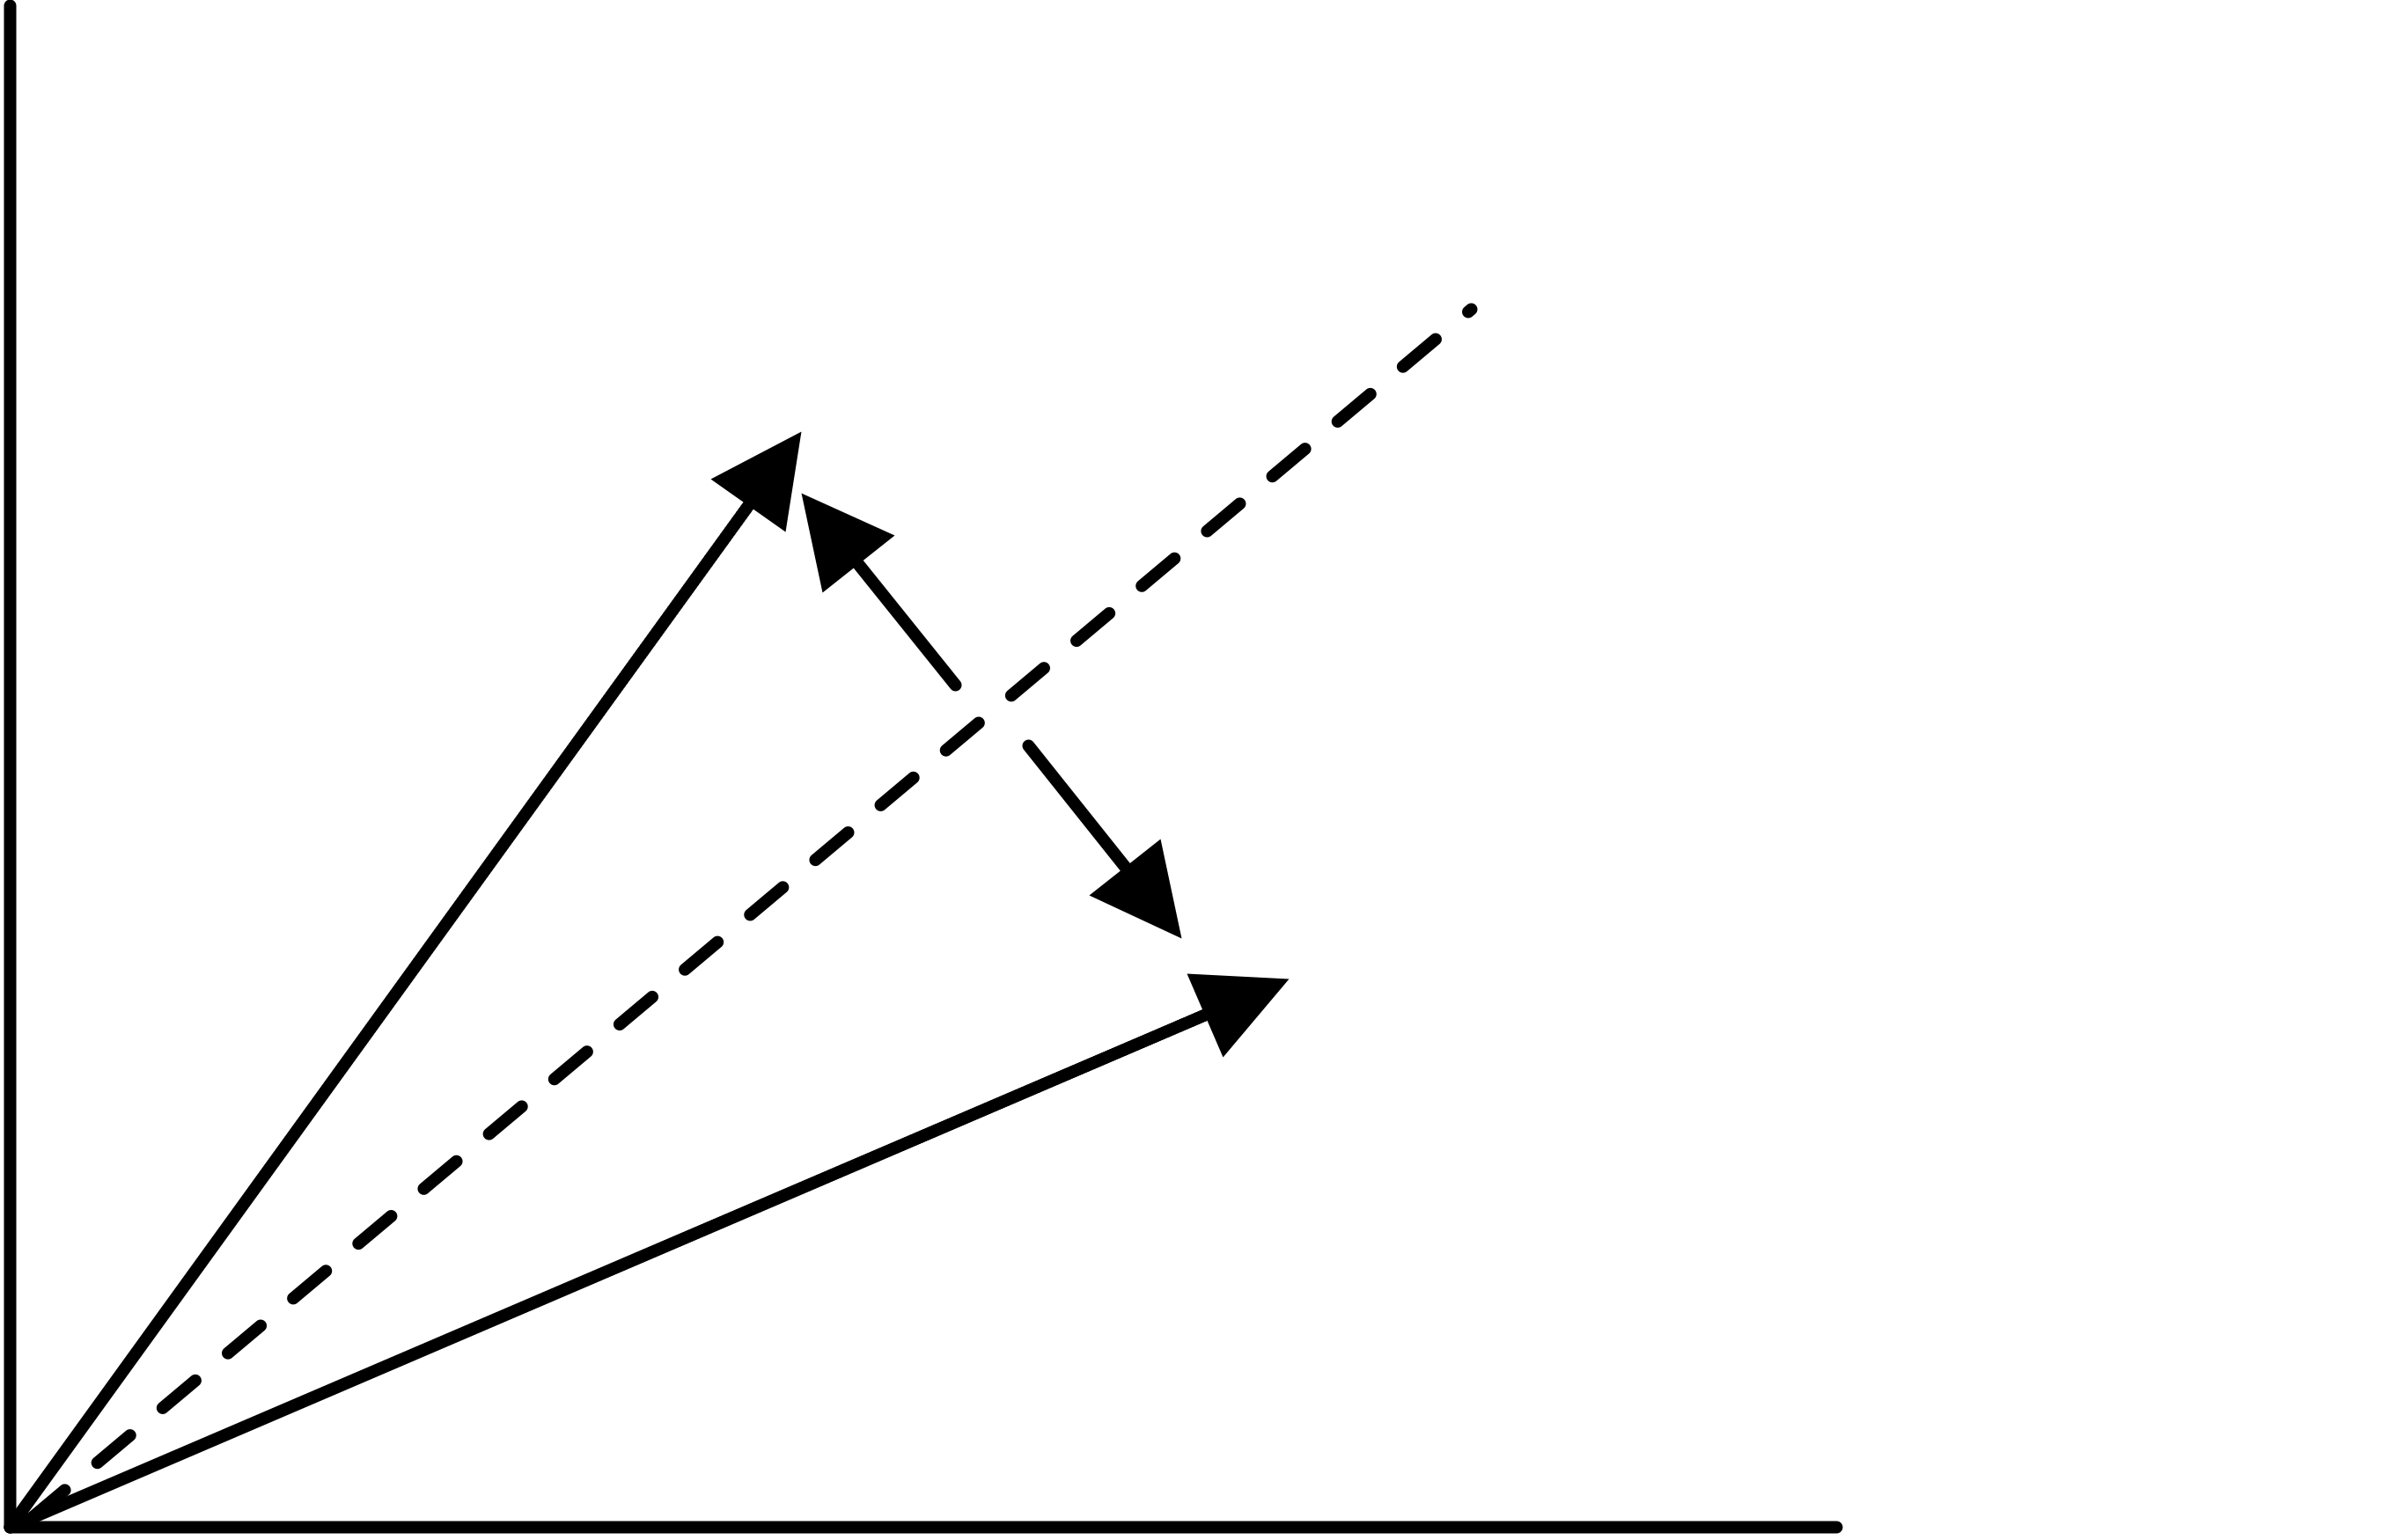
\includegraphics[scale=.1]{reflector}
  \caption{Householder reflector}
  \label{fig:reflector}
\end{figure}
In other words, we can map $x$ into~$y$ with the reflector based on
$u=(x-y)/2$.

We can generalize Householder reflectors to a form \[ H=I-2uv^t. \]
The matrices $L_i$ used in LU factorization (see section~\ref{sec:lu-fact})
can then be seen to be of the form $L_i = I-\ell_ie_i^t$ where $e_i$~has a single one
in the $i$-th location, and $\ell_i$~only has nonzero below that location.
That form also makes it easy to see that $L_i\inv = I+\ell_ie_i^t$:
\[ (I-uv^t)(I+uv^t) = I-uv^tuv^t = 0 \]
if $v^tu=0$.

\index{Householder reflectors|)}

